\chapter{Conceptos básicos de grafos}

Muchos problemas de programación se pueden resolver
modelando el problema como un problema de grafo
y utilizando un algoritmo de grafo adecuado.
Un ejemplo típico de grafo es una red
de carreteras y ciudades en un país.
A veces, sin embargo, el grafo está oculto
en el problema y puede ser difícil de detectarlo.

Esta parte del libro discute los algoritmos de grafos,
especialmente centrándose en temas que
son importantes en la programación competitiva.
En este capítulo, repasamos conceptos
relacionados con grafos,
y estudiamos diferentes formas de representar grafos en algoritmos.

\section{Terminología de grafos}

\index{grafo}
\index{nodo}
\index{arista}

Un \key{grafo} consta de \key{nodos}
y \key{aristas}. En este libro,
la variable $n$ denota el número de nodos
en un grafo, y la variable $m$ denota
el número de aristas.
Los nodos están numerados
usando números enteros $1,2,\ldots,n$.

Por ejemplo, el siguiente grafo consta de 5 nodos y 7 aristas:

\begin{center}
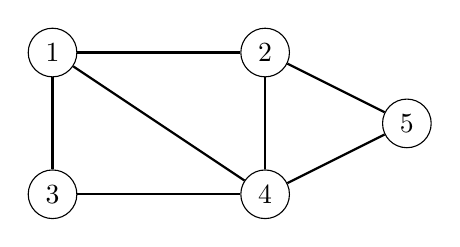
\begin{tikzpicture}[scale=0.9]
\node[draw, circle] (1) at (1,3) {$1$};
\node[draw, circle] (2) at (4,3) {$2$};
\node[draw, circle] (3) at (1,1) {$3$};
\node[draw, circle] (4) at (4,1) {$4$};
\node[draw, circle] (5) at (6,2) {$5$};

\path[draw,thick,-] (1) -- (2);
\path[draw,thick,-] (1) -- (3);
\path[draw,thick,-] (1) -- (4);
\path[draw,thick,-] (3) -- (4);
\path[draw,thick,-] (2) -- (4);
\path[draw,thick,-] (2) -- (5);
\path[draw,thick,-] (4) -- (5);
\end{tikzpicture}
\end{center}

\index{camino}

Un \key{camino} va del nodo $a$ al nodo $b$
a través de aristas del grafo.
La \key{longitud} de un camino es el número de
aristas en él.
Por ejemplo, el grafo anterior contiene
un camino $1 \rightarrow 3 \rightarrow 4 \rightarrow 5$
de longitud 3
desde el nodo 1 al nodo 5:

\begin{center}
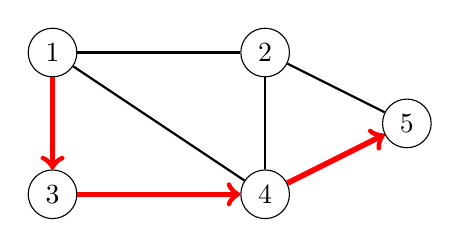
\begin{tikzpicture}[scale=0.9]
\node[draw, circle] (1) at (1,3) {$1$};
\node[draw, circle] (2) at (4,3) {$2$};
\node[draw, circle] (3) at (1,1) {$3$};
\node[draw, circle] (4) at (4,1) {$4$};
\node[draw, circle] (5) at (6,2) {$5$};

\path[draw,thick,-] (1) -- (2);
\path[draw,thick,-] (1) -- (3);
\path[draw,thick,-] (1) -- (4);
\path[draw,thick,-] (3) -- (4);
\path[draw,thick,-] (2) -- (4);
\path[draw,thick,-] (2) -- (5);
\path[draw,thick,-] (4) -- (5);

\path[draw=red,thick,->,line width=2pt] (1) -- (3);
\path[draw=red,thick,->,line width=2pt] (3) -- (4);
\path[draw=red,thick,->,line width=2pt] (4) -- (5);
\end{tikzpicture}
\end{center}

\index{ciclo}

Un camino es un \key{ciclo} si el primer y último
nodo es el mismo.
Por ejemplo, el grafo anterior contiene
un ciclo $1 \rightarrow 3 \rightarrow 4 \rightarrow 1$.
Un camino es \key{simple} si cada nodo aparece
a lo sumo una vez en el camino.


% 
% \begin{itemize}
% \item $1 \rightarrow 2 \rightarrow 5$ (length 2)
% \item $1 \rightarrow 4 \rightarrow 5$ (length 2)
% \item $1 \rightarrow 2 \rightarrow 4 \rightarrow 5$ (length 3)
% \item $1 \rightarrow 3 \rightarrow 4 \rightarrow 5$ (length 3)
% \item $1 \rightarrow 4 \rightarrow 2 \rightarrow 5$ (length 3)
% \item $1 \rightarrow 3 \rightarrow 4 \rightarrow 2 \rightarrow 5$ (length 4)
% \end{itemize}

\subsubsection{Conectividad}

\index{grafo conectado}

Un grafo es \key{conectado} si hay un camino
entre cualquier par de nodos.
Por ejemplo, el siguiente grafo está conectado:
\begin{center}
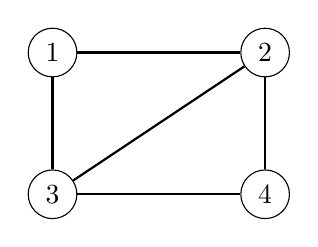
\begin{tikzpicture}[scale=0.9]
\node[draw, circle] (1) at (1,3) {$1$};
\node[draw, circle] (2) at (4,3) {$2$};
\node[draw, circle] (3) at (1,1) {$3$};
\node[draw, circle] (4) at (4,1) {$4$};
\path[draw,thick,-] (1) -- (2);
\path[draw,thick,-] (1) -- (3);
\path[draw,thick,-] (2) -- (3);
\path[draw,thick,-] (3) -- (4);
\path[draw,thick,-] (2) -- (4);
\end{tikzpicture}
\end{center}

El siguiente grafo no está conectado,
porque no es posible llegar
desde el nodo 4 a cualquier otro nodo:
\begin{center}
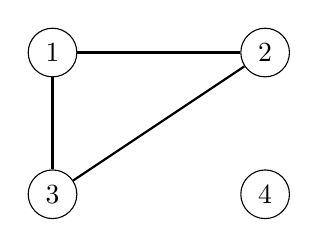
\begin{tikzpicture}[scale=0.9]
\node[draw, circle] (1) at (1,3) {$1$};
\node[draw, circle] (2) at (4,3) {$2$};
\node[draw, circle] (3) at (1,1) {$3$};
\node[draw, circle] (4) at (4,1) {$4$};
\path[draw,thick,-] (1) -- (2);
\path[draw,thick,-] (1) -- (3);
\path[draw,thick,-] (2) -- (3);
\end{tikzpicture}
\end{center}

\index{componente}

Las partes conectadas de un grafo son
llamadas sus \key{componentes}.
Por ejemplo, el siguiente grafo
contiene tres componentes:
$\{1,\,2,\,3\}$,
$\{4,\,5,\,6,\,7\}$ y
$\{8\}$.
\begin{center}
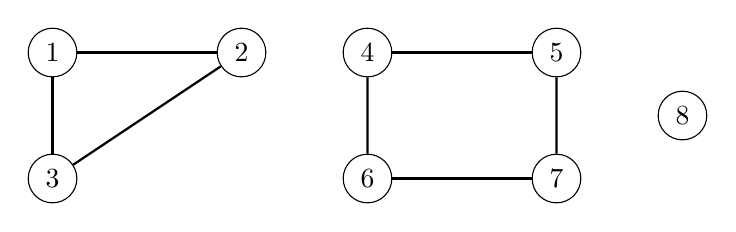
\begin{tikzpicture}[scale=0.8]
\node[draw, circle] (1) at (1,3) {$1$};
\node[draw, circle] (2) at (4,3) {$2$};
\node[draw, circle] (3) at (1,1) {$3$};

\node[draw, circle] (6) at (6,1) {$6$};
\node[draw, circle] (7) at (9,1) {$7$};
\node[draw, circle] (4) at (6,3) {$4$};
\node[draw, circle] (5) at (9,3) {$5$};

\node[draw, circle] (8) at (11,2) {$8$};

\path[draw,thick,-] (1) -- (2);
\path[draw,thick,-] (2) -- (3);
\path[draw,thick,-] (1) -- (3);
\path[draw,thick,-] (4) -- (5);
\path[draw,thick,-] (5) -- (7);
\path[draw,thick,-] (6) -- (7);
\path[draw,thick,-] (6) -- (4);
\end{tikzpicture}
\end{center}

\index{árbol}

Un \key{árbol} es un grafo conectado
que consta de $n$ nodos y $n-1$ aristas.
Hay un camino único
entre cualquier par de nodos de un árbol.
Por ejemplo, el siguiente grafo es un árbol:

\begin{center}
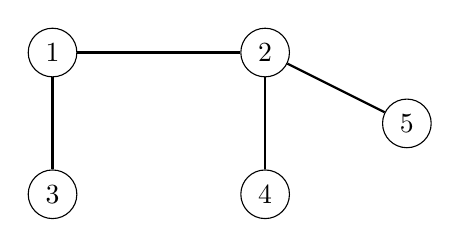
\begin{tikzpicture}[scale=0.9]
\node[draw, circle] (1) at (1,3) {$1$};
\node[draw, circle] (2) at (4,3) {$2$};
\node[draw, circle] (3) at (1,1) {$3$};
\node[draw, circle] (4) at (4,1) {$4$};
\node[draw, circle] (5) at (6,2) {$5$};

\path[draw,thick,-] (1) -- (2);
\path[draw,thick,-] (1) -- (3);
%\path[draw,thick,-] (1) -- (4);
\path[draw,thick,-] (2) -- (5);
\path[draw,thick,-] (2) -- (4);
%\path[draw,thick,-] (4) -- (5);
\end{tikzpicture}
\end{center}

\subsubsection{Direcciones de las aristas}

\index{grafo dirigido}

Un grafo es \key{dirigido}
si las aristas se pueden recorrer
solo en una dirección.
Por ejemplo, el siguiente grafo es dirigido:
\begin{center}
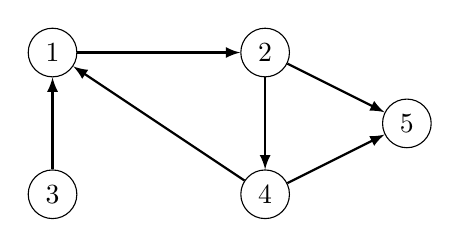
\begin{tikzpicture}[scale=0.9]
\node[draw, circle] (1) at (1,3) {$1$};
\node[draw, circle] (2) at (4,3) {$2$};
\node[draw, circle] (3) at (1,1) {$3$};
\node[draw, circle] (4) at (4,1) {$4$};
\node[draw, circle] (5) at (6,2) {$5$};
\path[draw,thick,->,>=latex] (1) -- (2);
\path[draw,thick,->,>=latex] (2) -- (4);
\path[draw,thick,->,>=latex] (2) -- (5);
\path[draw,thick,->,>=latex] (4) -- (5);
\path[draw,thick,->,>=latex] (4) -- (1);
\path[draw,thick,->,>=latex] (3) -- (1);
\end{tikzpicture}
\end{center}

El grafo anterior contiene
un camino $3 \rightarrow 1 \rightarrow 2 \rightarrow 5$
desde el nodo $3$ hasta el nodo $5$,
pero no hay un camino desde el nodo $5$ hasta el nodo $3$.

\subsubsection{Pesos de las aristas}

\index{grafo ponderado}

En un \key{grafo ponderado}, a cada arista se le asigna
un \key{peso}.
Los pesos a menudo se interpretan como longitudes de arista.
Por ejemplo, el siguiente grafo es ponderado:
\begin{center}
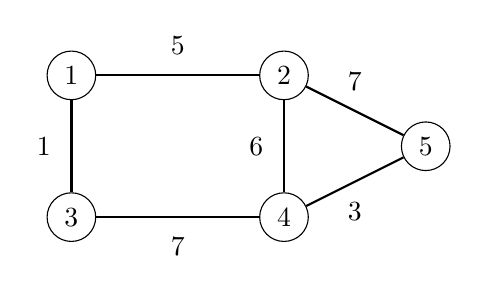
\begin{tikzpicture}[scale=0.9]
\node[draw, circle] (1) at (1,3) {$1$};
\node[draw, circle] (2) at (4,3) {$2$};
\node[draw, circle] (3) at (1,1) {$3$};
\node[draw, circle] (4) at (4,1) {$4$};
\node[draw, circle] (5) at (6,2) {$5$};
\path[draw,thick,-] (1) -- node[font=\small,label=above:5] {} (2);
\path[draw,thick,-] (1) -- node[font=\small,label=left:1] {} (3);
\path[draw,thick,-] (3) -- node[font=\small,label=below:7] {} (4);
\path[draw,thick,-] (2) -- node[font=\small,label=left:6] {} (4);
\path[draw,thick,-] (2) -- node[font=\small,label=above:7] {} (5);
\path[draw,thick,-] (4) -- node[font=\small,label=below:3] {} (5);
\end{tikzpicture}
\end{center}

La longitud de un camino en un grafo ponderado
es la suma de los pesos de las aristas en el camino.
Por ejemplo, en el grafo anterior,
la longitud del camino
$1 \rightarrow 2 \rightarrow 5$ es $12$,
y la longitud del camino
$1 \rightarrow 3 \rightarrow 4 \rightarrow 5$ es $11$.
Este último camino es el \key{más corto} desde el nodo $1$ hasta el nodo $5$.

\subsubsection{Vecinos y grados}

\index{vecino}
\index{grado}

Dos nodos son \key{vecinos} o \key{adyacentes}
si hay una arista entre ellos.
El \key{grado} de un nodo
es el número de sus vecinos.
Por ejemplo, en el siguiente grafo,
los vecinos del nodo 2 son 1, 4 y 5,
por lo que su grado es 3.

\begin{center}
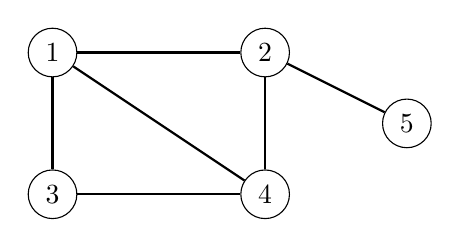
\begin{tikzpicture}[scale=0.9]
\node[draw, circle] (1) at (1,3) {$1$};
\node[draw, circle] (2) at (4,3) {$2$};
\node[draw, circle] (3) at (1,1) {$3$};
\node[draw, circle] (4) at (4,1) {$4$};
\node[draw, circle] (5) at (6,2) {$5$};

\path[draw,thick,-] (1) -- (2);
\path[draw,thick,-] (1) -- (3);
\path[draw,thick,-] (1) -- (4);
\path[draw,thick,-] (3) -- (4);
\path[draw,thick,-] (2) -- (4);
\path[draw,thick,-] (2) -- (5);
%\path[draw,thick,-] (4) -- (5);
\end{tikzpicture}
\end{center}

La suma de los grados en un grafo siempre es $2m$,
donde $m$ es el número de aristas,
porque cada arista
aumenta el grado de exactamente dos nodos en uno.
Por esta razón, la suma de los grados siempre es par.

\index{grafo regular}
\index{grafo completo}

Un grafo es \key{regular} si el
grado de cada nodo es una constante $d$.
Un grafo es \key{completo} si el
grado de cada nodo es $n-1$, es decir,
el grafo contiene todas las aristas posibles
entre los nodos.

\index{grado de entrada}
\index{grado de salida}

En un grafo dirigido, el \key{grado de entrada}
de un nodo es el número de aristas
que terminan en el nodo,
y el \key{grado de salida} de un nodo
es el número de aristas que comienzan en el nodo.
Por ejemplo, en el siguiente grafo,
el grado de entrada del nodo 2 es 2,
y el grado de salida del nodo 2 es 1.

\begin{center}
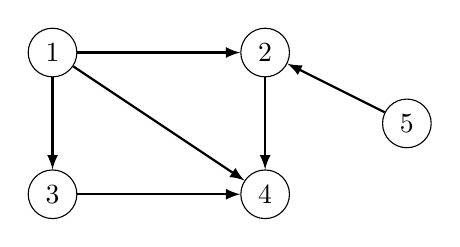
\begin{tikzpicture}[scale=0.9]
\node[draw, circle] (1) at (1,3) {$1$};
\node[draw, circle] (2) at (4,3) {$2$};
\node[draw, circle] (3) at (1,1) {$3$};
\node[draw, circle] (4) at (4,1) {$4$};
\node[draw, circle] (5) at (6,2) {$5$};

\path[draw,thick,->,>=latex] (1) -- (2);
\path[draw,thick,->,>=latex] (1) -- (3);
\path[draw,thick,->,>=latex] (1) -- (4);
\path[draw,thick,->,>=latex] (3) -- (4);
\path[draw,thick,->,>=latex] (2) -- (4);
\path[draw,thick,<-,>=latex] (2) -- (5);
\end{tikzpicture}
\end{center}

\subsubsection{Coloración}

\index{coloración}
\index{grafo bipartito}

En una \key{coloración} de un grafo,
a cada nodo se le asigna un color de tal manera que
no haya nodos adyacentes del mismo color.

Un grafo es \key{bipartito} si
es posible colorearlo usando dos colores.
Resulta que un grafo es bipartito
exactamente cuando no contiene un ciclo
con un número impar de aristas.
Por ejemplo, el grafo
\begin{center}
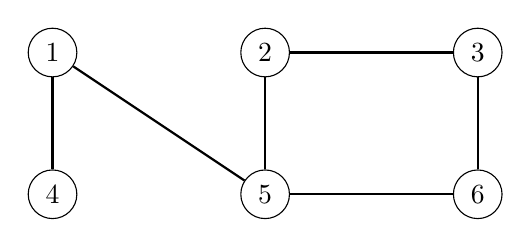
\begin{tikzpicture}[scale=0.9]
\node[draw, circle] (1) at (1,3) {$2$};
\node[draw, circle] (2) at (4,3) {$3$};
\node[draw, circle] (3) at (1,1) {$5$};
\node[draw, circle] (4) at (4,1) {$6$};
\node[draw, circle] (5) at (-2,1) {$4$};
\node[draw, circle] (6) at (-2,3) {$1$};
\path[draw,thick,-] (1) -- (2);
\path[draw,thick,-] (1) -- (3);
\path[draw,thick,-] (3) -- (4);
\path[draw,thick,-] (2) -- (4);
\path[draw,thick,-] (3) -- (6);
\path[draw,thick,-] (5) -- (6);
\end{tikzpicture}
\end{center}
es bipartito, porque se puede colorear de la siguiente manera:
\begin{center}
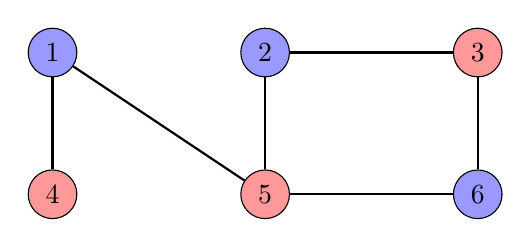
\begin{tikzpicture}[scale=0.9]
\node[draw, circle, fill=blue!40] (1) at (1,3) {$2$};
\node[draw, circle, fill=red!40] (2) at (4,3) {$3$};
\node[draw, circle, fill=red!40] (3) at (1,1) {$5$};
\node[draw, circle, fill=blue!40] (4) at (4,1) {$6$};
\node[draw, circle, fill=red!40] (5) at (-2,1) {$4$};
\node[draw, circle, fill=blue!40] (6) at (-2,3) {$1$};
\path[draw,thick,-] (1) -- (2);
\path[draw,thick,-] (1) -- (3);
\path[draw,thick,-] (3) -- (4);
\path[draw,thick,-] (2) -- (4);
\path[draw,thick,-] (3) -- (6);
\path[draw,thick,-] (5) -- (6);
\end{tikzpicture}
\end{center}
Sin embargo, el grafo
\begin{center}
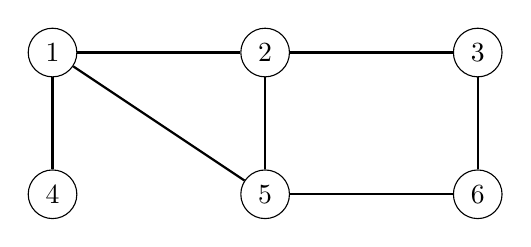
\begin{tikzpicture}[scale=0.9]
\node[draw, circle] (1) at (1,3) {$2$};
\node[draw, circle] (2) at (4,3) {$3$};
\node[draw, circle] (3) at (1,1) {$5$};
\node[draw, circle] (4) at (4,1) {$6$};
\node[draw, circle] (5) at (-2,1) {$4$};
\node[draw, circle] (6) at (-2,3) {$1$};
\path[draw,thick,-] (1) -- (2);
\path[draw,thick,-] (1) -- (3);
\path[draw,thick,-] (3) -- (4);
\path[draw,thick,-] (2) -- (4);
\path[draw,thick,-] (3) -- (6);
\path[draw,thick,-] (5) -- (6);
\path[draw,thick,-] (1) -- (6);
\end{tikzpicture}
\end{center}
no es bipartito, porque no es posible colorear
el siguiente ciclo de tres nodos usando dos colores:
\begin{center}
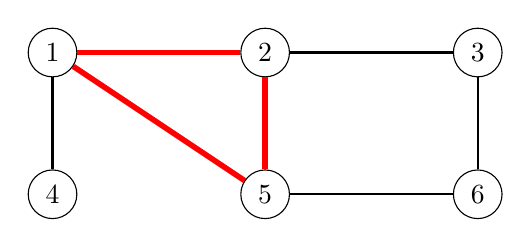
\begin{tikzpicture}[scale=0.9]
\node[draw, circle] (1) at (1,3) {$2$};
\node[draw, circle] (2) at (4,3) {$3$};
\node[draw, circle] (3) at (1,1) {$5$};
\node[draw, circle] (4) at (4,1) {$6$};
\node[draw, circle] (5) at (-2,1) {$4$};
\node[draw, circle] (6) at (-2,3) {$1$};
\path[draw,thick,-] (1) -- (2);
\path[draw,thick,-] (1) -- (3);
\path[draw,thick,-] (3) -- (4);
\path[draw,thick,-] (2) -- (4);
\path[draw,thick,-] (3) -- (6);
\path[draw,thick,-] (5) -- (6);
\path[draw,thick,-] (1) -- (6);

\path[draw=red,thick,-,line width=2pt] (1) -- (3);
\path[draw=red,thick,-,line width=2pt] (3) -- (6);
\path[draw=red,thick,-,line width=2pt] (6) -- (1);
\end{tikzpicture}
\end{center}

\subsubsection{Simplicidad}

\index{grafo simple}

Un grafo es \key{simple}
si ninguna arista comienza y termina en el mismo nodo,
y no hay múltiples
aristas entre dos nodos.
A menudo, asumimos que los grafos son simples.
Por ejemplo, el siguiente grafo \emph{no} es simple:
\begin{center}
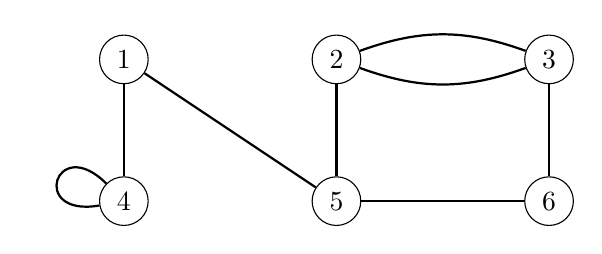
\begin{tikzpicture}[scale=0.9]
\node[draw, circle] (1) at (1,3) {$2$};
\node[draw, circle] (2) at (4,3) {$3$};
\node[draw, circle] (3) at (1,1) {$5$};
\node[draw, circle] (4) at (4,1) {$6$};
\node[draw, circle] (5) at (-2,1) {$4$};
\node[draw, circle] (6) at (-2,3) {$1$};

\path[draw,thick,-] (1) edge [bend right=20] (2);
\path[draw,thick,-] (2) edge [bend right=20] (1);
%\path[draw,thick,-] (1) -- (2);
\path[draw,thick,-] (1) -- (3);
\path[draw,thick,-] (3) -- (4);
\path[draw,thick,-] (2) -- (4);
\path[draw,thick,-] (3) -- (6);
\path[draw,thick,-] (5) -- (6);

\tikzset{every loop/.style={in=135,out=190}}
\path[draw,thick,-] (5) edge [loop left] (5);
\end{tikzpicture}
\end{center}

\section{Representación de grafos}

Existen varias formas de representar grafos
en algoritmos.
La elección de una estructura de datos
depende del tamaño del grafo y
de la forma en que el algoritmo lo procesa.
A continuación, veremos tres representaciones comunes.

\subsubsection{Representación por lista de adyacencia}

\index{lista de adyacencia}

En la representación por lista de adyacencia,
a cada nodo $x$ del grafo se le asigna una \key{lista de adyacencia}
que consiste en los nodos
a los que hay una arista desde $x$.
Las listas de adyacencia son la forma más popular
de representar grafos, y la mayoría de los algoritmos pueden ser
implementados de manera eficiente utilizando esta estructura.

Una forma conveniente de almacenar las listas de adyacencia es declarar
un arreglo de vectores de la siguiente forma:
\begin{lstlisting}
vector<int> adj[N];
\end{lstlisting}

La constante $N$ se elige de forma que se puedan almacenar todas
las listas de adyacencia.
Por ejemplo, el grafo

\begin{center}
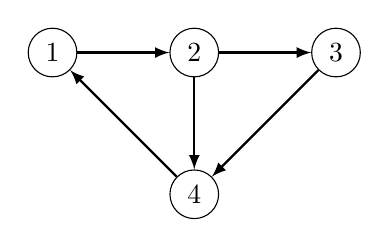
\begin{tikzpicture}[scale=0.9]
\node[draw, circle] (1) at (1,3) {$1$};
\node[draw, circle] (2) at (3,3) {$2$};
\node[draw, circle] (3) at (5,3) {$3$};
\node[draw, circle] (4) at (3,1) {$4$};

\path[draw,thick,->,>=latex] (1) -- (2);
\path[draw,thick,->,>=latex] (2) -- (3);
\path[draw,thick,->,>=latex] (2) -- (4);
\path[draw,thick,->,>=latex] (3) -- (4);
\path[draw,thick,->,>=latex] (4) -- (1);
\end{tikzpicture}
\end{center}
puede almacenarse de la siguiente manera:
\begin{lstlisting}
adj[1].push_back(2);
adj[2].push_back(3);
adj[2].push_back(4);
adj[3].push_back(4);
adj[4].push_back(1);
\end{lstlisting}

Si el grafo es no dirigido, se puede almacenar de manera similar,
pero cada arista se agrega en ambas direcciones.

Para un grafo ponderado, la estructura se puede extender
de la siguiente manera:

\begin{lstlisting}
vector<pair<int,int>> adj[N];
\end{lstlisting}

En este caso, la lista de adyacencia del nodo $a$
contiene el par $(b,w)$
siempre que haya una arista desde el nodo $a$ hacia el nodo $b$
con peso $w$. Por ejemplo, el grafo

\begin{center}
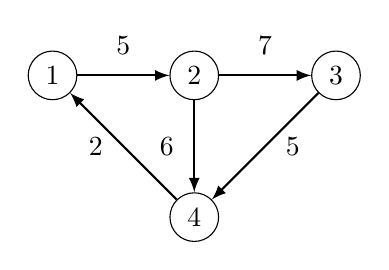
\begin{tikzpicture}[scale=0.9]
\node[draw, circle] (1) at (1,3) {$1$};
\node[draw, circle] (2) at (3,3) {$2$};
\node[draw, circle] (3) at (5,3) {$3$};
\node[draw, circle] (4) at (3,1) {$4$};

\path[draw,thick,->,>=latex] (1) -- node[font=\small,label=above:5] {} (2);
\path[draw,thick,->,>=latex] (2) -- node[font=\small,label=above:7] {} (3);
\path[draw,thick,->,>=latex] (2) -- node[font=\small,label=left:6] {} (4);
\path[draw,thick,->,>=latex] (3) -- node[font=\small,label=right:5] {} (4);
\path[draw,thick,->,>=latex] (4) -- node[font=\small,label=left:2] {} (1);
\end{tikzpicture}
\end{center}
puede almacenarse de la siguiente manera:
\begin{lstlisting}
adj[1].push_back({2,5});
adj[2].push_back({3,7});
adj[2].push_back({4,6});
adj[3].push_back({4,5});
adj[4].push_back({1,2});
\end{lstlisting}

El beneficio de utilizar listas de adyacencia es que
podemos encontrar de manera eficiente los nodos a los que
podemos movernos desde un nodo dado a través de una arista.
Por ejemplo, el siguiente ciclo recorre todos los nodos
a los que podemos movernos desde el nodo $s$:

\begin{lstlisting}
for (auto u : adj[s]) {
    // procesar el nodo u
}
\end{lstlisting}

\subsubsection{Representación por matriz de adyacencia}

\index{matriz de adyacencia}

Una \key{matriz de adyacencia} es un arreglo bidimensional
que indica qué aristas contiene el grafo.
Podemos verificar de manera eficiente desde una matriz de adyacencia
si hay una arista entre dos nodos.
La matriz puede almacenarse como un arreglo
\begin{lstlisting}
int adj[N][N];
\end{lstlisting}
donde cada valor $\texttt{adj}[a][b]$ indica
si el grafo contiene una arista desde
el nodo $a$ al nodo $b$.
Si la arista está presente en el grafo,
entonces $\texttt{adj}[a][b]=1$,
y si no está presente, $\texttt{adj}[a][b]=0$.
Por ejemplo, el grafo
\begin{center}
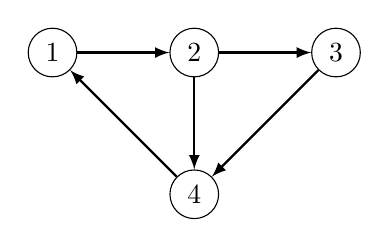
\begin{tikzpicture}[scale=0.9]
\node[draw, circle] (1) at (1,3) {$1$};
\node[draw, circle] (2) at (3,3) {$2$};
\node[draw, circle] (3) at (5,3) {$3$};
\node[draw, circle] (4) at (3,1) {$4$};

\path[draw,thick,->,>=latex] (1) -- (2);
\path[draw,thick,->,>=latex] (2) -- (3);
\path[draw,thick,->,>=latex] (2) -- (4);
\path[draw,thick,->,>=latex] (3) -- (4);
\path[draw,thick,->,>=latex] (4) -- (1);
\end{tikzpicture}
\end{center}
puede representarse de la siguiente manera:
\begin{center}
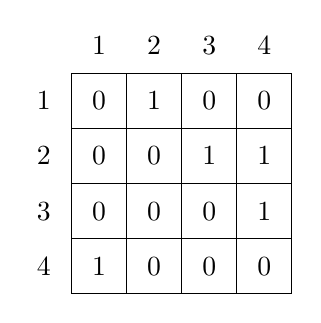
\begin{tikzpicture}[scale=0.7]
\draw (0,0) grid (4,4);
\node at (0.5,0.5) {1};
\node at (1.5,0.5) {0};
\node at (2.5,0.5) {0};
\node at (3.5,0.5) {0};
\node at (0.5,1.5) {0};
\node at (1.5,1.5) {0};
\node at (2.5,1.5) {0};
\node at (3.5,1.5) {1};
\node at (0.5,2.5) {0};
\node at (1.5,2.5) {0};
\node at (2.5,2.5) {1};
\node at (3.5,2.5) {1};
\node at (0.5,3.5) {0};
\node at (1.5,3.5) {1};
\node at (2.5,3.5) {0};
\node at (3.5,3.5) {0};
\node at (-0.5,0.5) {4};
\node at (-0.5,1.5) {3};
\node at (-0.5,2.5) {2};
\node at (-0.5,3.5) {1};
\node at (0.5,4.5) {1};
\node at (1.5,4.5) {2};
\node at (2.5,4.5) {3};
\node at (3.5,4.5) {4};
\end{tikzpicture}
\end{center}

Si el grafo es ponderado, la representación de la matriz de adyacencia
puede extenderse para que
la matriz contenga el peso de la arista
si existe la arista.
Usando esta representación, el grafo

\begin{center}
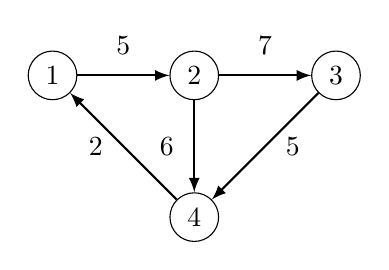
\begin{tikzpicture}[scale=0.9]
\node[draw, circle] (1) at (1,3) {$1$};
\node[draw, circle] (2) at (3,3) {$2$};
\node[draw, circle] (3) at (5,3) {$3$};
\node[draw, circle] (4) at (3,1) {$4$};

\path[draw,thick,->,>=latex] (1) -- node[font=\small,label=above:5] {} (2);
\path[draw,thick,->,>=latex] (2) -- node[font=\small,label=above:7] {} (3);
\path[draw,thick,->,>=latex] (2) -- node[font=\small,label=left:6] {} (4);
\path[draw,thick,->,>=latex] (3) -- node[font=\small,label=right:5] {} (4);
\path[draw,thick,->,>=latex] (4) -- node[font=\small,label=left:2] {} (1);
\end{tikzpicture}
\end{center}
\begin{samepage}
corresponde a la siguiente matriz:
\begin{center}
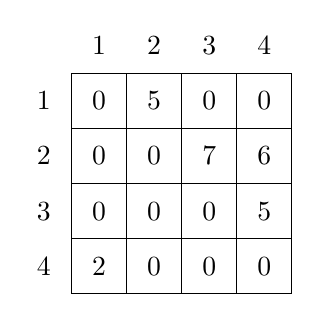
\begin{tikzpicture}[scale=0.7]
\draw (0,0) grid (4,4);
\node at (0.5,0.5) {2};
\node at (1.5,0.5) {0};
\node at (2.5,0.5) {0};
\node at (3.5,0.5) {0};
\node at (0.5,1.5) {0};
\node at (1.5,1.5) {0};
\node at (2.5,1.5) {0};
\node at (3.5,1.5) {5};
\node at (0.5,2.5) {0};
\node at (1.5,2.5) {0};
\node at (2.5,2.5) {7};
\node at (3.5,2.5) {6};
\node at (0.5,3.5) {0};
\node at (1.5,3.5) {5};
\node at (2.5,3.5) {0};
\node at (3.5,3.5) {0};
\node at (-0.5,0.5) {4};
\node at (-0.5,1.5) {3};
\node at (-0.5,2.5) {2};
\node at (-0.5,3.5) {1};
\node at (0.5,4.5) {1};
\node at (1.5,4.5) {2};
\node at (2.5,4.5) {3};
\node at (3.5,4.5) {4};
\end{tikzpicture}
\end{center}
\end{samepage}

El inconveniente de la representación con la matriz de adyacencia
es que la matriz contiene $n^2$ elementos,
y usualmente la mayoría de ellos son ceros.
Por esta razón, la representación no puede usarse
si el grafo es grande.

\subsubsection{Representación por lista de aristas}

\index{lista de aristas}

Una \key{lista de aristas} contiene todas las aristas de un grafo
en algún orden.
Este es un modo conveniente de representar un grafo
si el algoritmo procesa todas las aristas del grafo
y no es necesario encontrar las aristas que parten
de un nodo dado.

La lista de aristas puede almacenarse en un vector
\begin{lstlisting}
vector<pair<int,int>> aristas;
\end{lstlisting}
donde cada par $(a,b)$ indica que
hay una arista desde el nodo $a$ al nodo $b$.
Así, el grafo

\begin{center}
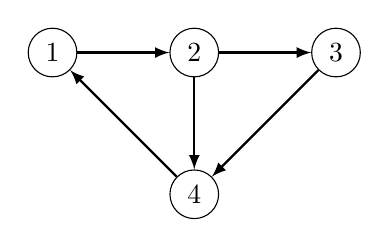
\begin{tikzpicture}[scale=0.9]
\node[draw, circle] (1) at (1,3) {$1$};
\node[draw, circle] (2) at (3,3) {$2$};
\node[draw, circle] (3) at (5,3) {$3$};
\node[draw, circle] (4) at (3,1) {$4$};

\path[draw,thick,->,>=latex] (1) -- (2);
\path[draw,thick,->,>=latex] (2) -- (3);
\path[draw,thick,->,>=latex] (2) -- (4);
\path[draw,thick,->,>=latex] (3) -- (4);
\path[draw,thick,->,>=latex] (4) -- (1);
\end{tikzpicture}
\end{center}
puede representarse como sigue:
\begin{lstlisting}
aristas.push_back({1,2});
aristas.push_back({2,3});
aristas.push_back({2,4});
aristas.push_back({3,4});
aristas.push_back({4,1});
\end{lstlisting}

\noindent
Si el grafo es ponderado, la estructura puede
ser extendida como sigue:
\begin{lstlisting}
vector<tuple<int,int,int>> aristas;
\end{lstlisting}
Cada elemento en esta lista tiene la
forma $(a,b,w)$, lo que significa que existe una
arista desde el nodo $a$ hasta el nodo $b$ con peso $w$.
Por ejemplo, el grafo

\begin{center}
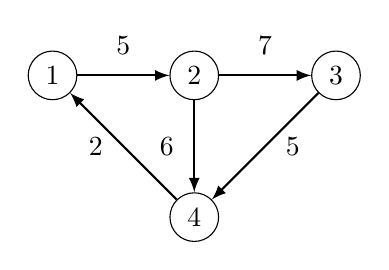
\begin{tikzpicture}[scale=0.9]
\node[draw, circle] (1) at (1,3) {$1$};
\node[draw, circle] (2) at (3,3) {$2$};
\node[draw, circle] (3) at (5,3) {$3$};
\node[draw, circle] (4) at (3,1) {$4$};

\path[draw,thick,->,>=latex] (1) -- node[font=\small,label=above:5] {} (2);
\path[draw,thick,->,>=latex] (2) -- node[font=\small,label=above:7] {} (3);
\path[draw,thick,->,>=latex] (2) -- node[font=\small,label=left:6] {} (4);
\path[draw,thick,->,>=latex] (3) -- node[font=\small,label=right:5] {} (4);
\path[draw,thick,->,>=latex] (4) -- node[font=\small,label=left:2] {} (1);
\end{tikzpicture}
\end{center}
\begin{samepage}
puede representarse como sigue\footnote{En algunos compiladores antiguos,
la función \texttt{make\_tuple} debe usarse en lugar de las llaves (por ejemplo,
\texttt{make\_tuple(1,2,5)} en lugar de \texttt{\{1,2,5\}}).}:
\begin{lstlisting}
aristas.push_back({1,2,5});
aristas.push_back({2,3,7});
aristas.push_back({2,4,6});
aristas.push_back({3,4,5});
aristas.push_back({4,1,2});
\end{lstlisting}
\end{samepage}
